
	\documentclass{article}
	\usepackage{amsmath,amssymb}
	\usepackage[inline]{enumitem}
	\usepackage{blindtext}
	\usepackage{booktabs}
	\usepackage{graphicx}
	\usepackage{xcolor}
	\usepackage[vmargin = 1.5in, top = 1in, bottom = 1.2in, letterpaper]{geometry}
	\usepackage{listings}
	\usepackage{courier}
	\usepackage{multicol}
	\usepackage{multirow}
	\usepackage{bm}
	\usepackage{diagbox}
	\usepackage{subcaption}
	\usepackage{tabularx}
	\lstset{
	basicstyle = \small\tt,
	keywordstyle = \tt\bfseries\color{blue},
	commentstyle = \it\color[cmyk]{1,0,1,0},
	stringstyle = \it\color[RGB]{128,0,0},
	%frame = single,
	backgroundcolor = \color[RGB]{245,245,244},
	breaklines,
	extendedchars = false,
	xleftmargin = 2em,
	xrightmargin = 2em,
	aboveskip = 1em,
	tabsize = 4,
	showspaces = false
	}
    \DeclareCaptionSubType * [alph]{table}
    \captionsetup[subtable]{labelformat=simple, labelsep=space}

    \renewcommand\thesubtable{\thetable(\alph{subtable})}

    \DeclareCaptionSubType * [alph]{figure}
    \captionsetup[subfigure]{labelformat=simple, labelsep=space}

    \renewcommand\thesubfigure{\thefigure(\alph{subfigure})}

	\begin{document}
	
	% \newfontfamily\courier{Courier New}

	
	\title{STAT 520 Exam 2}
	\author{Yifan Zhu}
	\maketitle
	\section{Introduction} % (fold)
	\label{sec:introduction}
	In this study, we want to compare the performance of 6 different confidence intervals when the data is from the Inverse Gaussian distribution. As the performance should vary with difference parameters of the distribution and the sampe size of the data, we conducted the comparison under 20 different situations, which are fixed $\mu = 5$ and a cross-classification of $n \in \{10, 25, 50, 100, 500\}$ and $\lambda \in \{2, 4, 8, 12\}$. The features to be compared about the confidence interval is the actual coverage rate, the median interval width and the probability of interval endpoints outside of a parameter space. If one kind of confidence interval has an actual coverage rate close to the desired coverage rate, small median interval width ,or low or no probability of its endpoints outside of the parameter space, we can say it is a good confidence interval in a specific situation. By doing this comparison, we would have an idea about which ones of the 6 kinds of confidence intervals are good in each situations. And the result of this study can give us a guide when we need to choose a method to get confidence intervals in specific situations in our future research.  
	

	\section{Description of Methods Used}
	\subsection{Algorithm outline}\label{outline}
    The outline of the algorithm for comparing 6 kinds of confidence intervals in the situation when true parameters are $(\mu, \lambda)$ and sample size is $n$ are as following:

    \begin{enumerate}
    	\item 
    	First with the Monte Carlo size $M$ we chose, we simulate $M$ samples of sample size $n$, denoted as $\{\bm y_m\}_{m=1}^M$. R function \verb|rinvgauss| from package \verb|statmod| is used to generate samples.

    	 \item 
    	 For each $\bm y_m$, we calculate these 6 kinds of confidence intervals. I wrote a function called \verb|intervals| that take each $\bm y_m$ as input and output 12 confidence intervals in a matrix, which are 2 confidence intervals for $\mu$ and $\lambda$ for each kind of 6 kinds of confidence interval. After the procedure goes through $m = 1,\ldots, M$, we now have $12 \times M$ confidence intervals, $M$ confidence intervals for each of $\mu$ and $\lambda$ and each kind of 6. 
         
         \item 
         With $M$ confidence intervals of a specific kind and for a specific parameter (e.g. $M$ confidence intervals based on MLE and Wald Theory for parameter $\mu$), we can then calculate the actual coverage rate, median interval width and probability of interval endpoints outside of a parameter space. 

         Function \verb|muiscovered| and \verb|lambdaiscovered| are written to determine whether a confidence interval covers the true $\mu$ and $\lambda$. The returned value is 1 for being covered and 0 for not being covered. We sum the returned values of \verb|muiscovered| or \verb|lambdaiscovered| over $m = 1, \ldots, M$ (depending on which of $\mu$ or $\lambda$ is that set of $M$ intervals corresponding to), we then have the total number a intervals that cover the true value. The total number of intervals covers true value divided by $M$ is then the actual coverage rate.

         Similarly, a function \verb|isout| is written to determine if the endpoints of a interval is outside of the parameter space. In this case, \verb|isout| returns 1 if the left endpoint is less than 0 and returns 0 otherwise. Then summing the returned values of \verb|isout| over $m = 1, \ldots, M$ and dividing it by $M$ gives us the probability of interval endpoints outside of a parameter space.

         To get the median interval width, function \verb|intwidth| is written to calculate the width of an interval for each of $M$ intervals. And then built-in function \verb|median| is used to get the median of the $M$ interval widths.  
    \end{enumerate}

    Now in a specific situation (fixed $n, \mu, \lambda$), we have the 3 features for each of the 6 kinds of intervals. Then we can compare how different kinds of intervals for $\mu$ and $\lambda$ performs under the given situation.
    
    In the remaining part of this section, we would elaborate how the function \verb|intervals| mentioned in Step 2 works. In fact it is a wrapper of several functions to calculate different kinds of intervals, which are \verb|muwaldint|, \verb|lambdawaldint|, \verb|muinvlikint|, \verb|lambdainvlikint|, \verb|bootmleints| and \verb|bootmmeints|. The MLE, estimated variance of MLE and MME of $\mu$ and $\lambda$ will be calculated first in \verb|intervals|, as these values will be used by the above functions one or more times. Functions named \verb|thetamle|, \verb|vthetamle| and \verb|thetamme| are written to calculate the MLE, estimated variance of MLE and MME for Inverse Gaussian distribution. The calculation of different kinds of intervals are shown in the following subsections.

	\subsection{MLE and Wald Theory}
    For Inverse Gaussian distribution, a good news for us is that we can actually obtain a simple closed form of MLE as well as the inverse of fisher information matrix. Let $\bm y = \{y_i\}_{i=1}^n$ be a sample from $IG(\mu, \lambda)$, then the log likelihood function is
    \[\ell_n (\mu, \lambda, \bm y) = \frac{n}{2} \log\left(\frac{\lambda}{2 \pi}\right) - \frac{3}{2}\log\left(\prod_{i=1}^n y_i\right) - \frac{\lambda}{2 \mu^2} \sum_{i=1}^n y_i + \frac{\lambda n}{\mu} - \frac{\lambda}{2} \sum_{i=1}^n \left(\frac{1}{y_i}\right)\]
    Let
    \begin{align*}
    &\frac{\partial \ell_n}{\partial \mu} = 0\\
    &\frac{\partial \ell_n}{\partial \lambda} = 0
    \end{align*}
    We have
    \begin{align*}
    & \hat{\mu}_n = \frac{\sum_{i=1}^n y_i}{n}\\
    & \hat{\lambda}_n = \frac{n}{\sum_{i=1}^n \left(\frac{1}{y_i} - \frac{1}{\hat{\mu}_n}\right)}
    \end{align*}
    And we can check these are indeed MLE that maximize the log likelihood.

    The inverse fisher information matrix is 
    \[I_n^{-1} = \begin{bmatrix}
    	\frac{\mu^3}{\lambda n} & 0 \\
    	0 & \frac{2 \lambda^2}{n}
    \end{bmatrix}\]
    Thus the estimated variance of $\hat{\mu}_n$ and $\hat{\lambda}_n$ are
    \begin{align*}
    & \widehat{Var}(\hat{\mu}_n) = \frac{\hat{\mu}_n^3}{\hat{\lambda}_n n}\\
    & \widehat{Var}(\hat{\lambda}_n) = \frac{2 \hat{\lambda}_n}{n}
    \end{align*}
    Then the 95\% confidence Wald Theory confidence interval for $\mu$ and $\lambda$ are 
    \[\left(\hat{\mu}_n - 1.96 \sqrt{\widehat{Var}(\hat{\mu}_n)}, \hat{\mu}_n + 1.96 \sqrt{\widehat{Var}(\hat{\mu}_n)}\right)\]
    and
    \[\left(\hat{\lambda}_n - 1.96 \sqrt{\widehat{Var}(\hat{\lambda}_n)}, \hat{\lambda}_n + 1.96 \sqrt{\widehat{Var}(\hat{\lambda}_n)}\right)\]

    Function \verb|thetamle| takes each sample $\bm y$ as input to calculate $\hat{\mu}_n$ and $\hat{\lambda}_n$. \verb|vthetamle| takes $\hat{\mu}_n$ and $\hat{\lambda}_n$ as input to calculate $\widehat{Var}(\hat{\mu}_n)$ and $\widehat{Var}(\hat{\lambda}_n)$. Finally \verb|muwaldint| and \verb|lambdawaldint| take $(\hat{\mu}_n, \widehat{Var}(\hat{\mu}_n))$ and $(\hat{\lambda}_n, \widehat{Var}(\hat{\lambda}_n))$ as input to calculate the 95\% Wald Theory confidence intervals respectively.

    
	\subsection{MLE and inversion of LRT}
	The 95\% confidence interval for $\mu$ obtained from MLE and inversion of LRT is
	\[\{\mu : -2(\ell_n(\mu, \tilde{\lambda}_n, \bm y) - \ell_n(\hat{\mu}_n, \hat{\lambda}_n, \bm y)) \leq \chi_{1, 0.95}^2\}\]
	Here $\hat{\mu}_n, \hat{\lambda}_n$ are MLE for log likelihood $\ell_n(\mu, \lambda, \bm y)$, $\tilde{\lambda}_n$ is MLE for profiled log likelihood $\ell_{n}^p (\lambda, \bm y) = \ell_n(\mu, \lambda, \bm y)$ for fixed $\mu$. The closed form of $\tilde{\lambda}_n$ is given by
	\[\tilde{\lambda}_n = \frac{n}{\sum_{i=1}^n \left(\frac{y_i}{\mu^2} - \frac{2}{\mu} + \frac{1}{y_i}\right)}\]
	which is a function of $\mu$. Then to solve the inequality, we want to find two roots of the function of $\mu$, denoted $f(\mu)$
	\[f(\mu) = \ell_n(\hat{\mu}_n, \hat{\lambda}_n, \bm y) - \ell_n({\mu, \tilde{\lambda}_n}, \bm y) - \frac{\chi_{1,0.95}^2}{2}\]
	Two roots are obtained using built-in function \verb|uniroot|. The left root in searched in interval $(0, \hat{\mu}_n)$, and the right root in $(\hat{\mu}_n, \infty)$. In implementing, $\infty$ is replaced by 10 times the right bound of the Wald Theory interval obtained previously.

	Similarly, the 95\% confidence interval for $\lambda$ obtained from MLE and inversion of LRT is
	\[\{\lambda : -2(\ell_n( \tilde{\mu}_n, \lambda, \bm y) - \ell_n(\hat{\mu}_n, \hat{\lambda}_n, \bm y)) \leq \chi_{1, 0.95}^2\}\]
	where MLE of $\mu$ for profiled likelihood $\tilde{\mu}_n = \sum_{i=1}^n y_i/n$. Then the function to find root is
	\[g(\lambda) = \ell_n(\hat{\mu}_n, \hat{\lambda}_n, \bm y) - \ell_n({\tilde{\mu}_n, \lambda}, \bm y) - \frac{\chi_{1,0.95}^2}{2}\]
	Two roots are search using \verb|uniroot| in $(0, \hat{\lambda}_n)$ and $(\hat{\lambda}_n, \infty)$. 

	When $n$ is small, it is possible that \verb|uniroot| fails to find the right root in given interval. In this case we set the right bound to be $\infty$.

	\subsection{Bootstrap intervals based on MLE}
	As the three kinds of bootstrap intervals based on MLE can be calculated using the same set of bootstrapped samples and the MLEs from those samples, we decide to calculate them at the same time. 

	First, with the bootstrap size $M_1$ we chose, we generate $M_1$ samples of size $n$ from $IG(\hat{\mu}_n, \hat{\lambda}_n)$. $\hat{\mu}_n, \hat{\lambda}_n$ are MLEs from sample $\bm y_m$ here. And for each $\bm{y}_k^{*}, k = 1, \ldots, M_1$, we calculate the corresponding MLEs $\{\hat{\mu}_{n,k}^*\}_{k=1}^{M_1}$ and $\{\hat{\lambda}_{n,k}^*\}_{k = 1}^{M_1}$ with function \verb|thetamle| applied to every $\bm y_k^{*}$. We can also obtain $\{\widehat{Var}(\hat{\mu}_{n, k}^*)\}_{k=1}^{M_1}$ and  $\{\widehat{Var}(\hat{\lambda}_{n, k}^*)\}_{k=1}^{M_1}$ by applying function \verb|vthetamle| to  $\{\hat{\mu}_{n,k}^*\}_{k=1}^{M_1}$ and $\{\hat{\lambda}_{n,k}^*\}_{k = 1}^{M_1}$. With MLEs and estimated variance for NLEs from bootstrapped samples, we then have the 3 kinds of 95\% bootstrap confidence intervals 
	\begin{align*}
	& h(\theta, \hat{\theta}) = n^{1/2}(\hat{\theta}_n - \theta) \Rightarrow \left(2 \hat{\theta}_n - \theta_{n, [(M_1 + 1)/0.975]}^*, 2 \hat{\theta}_n - \theta_{n, [(M_1 + 1)/0.025]}^*\right)\\
	& h(\theta, \hat{\theta}) = n^{1/2}\left(\frac{\theta}{\hat{\theta}_n} - 1\right) \Rightarrow \left(\frac{\hat{\theta}_n^2}{\theta_{n, [(M_1 + 1)/0.975]}^*}, \frac{\hat{\theta}_n}{\theta_{n, [(M_1 + 1)/0.025]}^*}\right)\\
	& h(\theta, \hat{\theta}) = \frac{\hat{\theta}_n - \theta}{[V(\hat{\theta}_n)]^{1/2}} \Rightarrow \left(\hat{\theta}_n - [\widehat{Var}(\hat{\theta}_n)]^{1/2}\left(\frac{\theta_{n}^* - \hat{\theta}_n}{\widehat{Var}(\theta_n^*)}\right)_{[(M_1 +1)/0.975]}, \hat{\theta}_n - [\widehat{Var}(\hat{\theta}_n)]^{1/2}\left(\frac{\theta_{n}^* - \hat{\theta}_n}{\widehat{Var}(\theta_n^*)}\right)_{[(M_1 +1)/0.025]}\right)
	\end{align*}
	where $\theta = \mu, \lambda$.

	\subsection{Bootstrap interval based on MME}
	The only difference of bootstrap interval based on MME with that of MLE is we replace MLEs $\mu$ and $\lambda$ with MMEs of $\mu$ and $\lambda$ when generating bootstrapped samples and calculating the MMEs of $\mu$ and $\lambda$ for each sample instead of MLEs.

	The MMEs for $\mu$ and $\lambda$ are
	\begin{align*}
	 & \hat{\mu}_n = \frac{\sum_{i=1}^n y_i}{n}\\
	 & \hat{\lambda}_n = \frac{1}{\sum_{i=1}^n y_i^2/(n \hat{\mu}_n) - 1/\hat{\mu}_n}
	 \end{align*}

	 And the 95\% confidence interval is
	 \[\left(2 \hat{\theta}_n - \theta_{n, [(M_1 + 1)/0.975]}^*, 2 \hat{\theta}_n - \theta_{n, [(M_1 + 1)/0.025]}^*\right)\]
	  

	\subsection{Choosing Monte Carlo Size $M$}
	$M$ is a parameter we need to choose before we do this Monte Carlo study. We want to choose an $M$ that is appropriately big such that the quantities we are interested in converge with that $M$. We take the first method, i.e. Wald Theory interval, to examine the convergence of actual coverage rate when $M$ goes through $\{500, 1000, 2000, \ldots, 9000, 100000, 20000, 50000, 100000, 200000\}$ in 5 different situations. The 5 situations we select are $\{(n, \lambda): (10, 2), (10, 12), (100, 4), (500, 2), (500,12)\}$. We look at the MC approximate of the actual coverage rate and its MC Interval width. In this way we determine a common $M$ to use in this whole study that guarantees the convergence of all the MC approximated values. Function \verb|interval_wald| that takes $\bm y_m$ as input is written to only return the Wald Theory intervals for $\mu$ and $\lambda$. Function \verb|rinvgauss| from \verb|statmod| is used to generate $\{\bm y_m: m = 1, \ldots, M\}. $ And the functions \verb|muiscovered| and \verb|lambdaiscovered| mentioned in section \ref{outline} is also used in this procedure to get the MC approximation of actual coverage rate.   

	\subsection{Chooing Bootstrap Size $M_1$}
	We also need the bootstrap size $M_1$ as a constant through the study that guarantees the convergence of bootstrap intervals through the study. Now we fix a sample $\bm y_0$ and for each $M_1 \in \{50, 100, 150, \ldots, 9050, 100000\}$, we use this sample to calculate the bootstrap interval width as a feature by the comparison function $n^{1/2}(\hat{\theta}_n - \theta)$ to check the convergence. We examine the change of interval width as $M_1$ goes larger by plotting the interval width against $M_1$.  We look at 6 different situations, which are $\{(n, \lambda): (10, 2), (10, 12), (50, 8), (100, 4), (500, 2), (500, 12)\}$. Then we want to find the appropriate $M_1$ that leads to the convergence of interval width in all situations, and then use this $M_1$ in the calculation of bootstrap intervals through the whole study. Function \verb|rinvgauss| is used to generate $\bm y_0$. And a function \verb|boot1ciwidth| is used to calculate the interval width.       

	\section{Results}
	\subsection{Choosing $M$}
	The results of convergence rate for different $M$s are presented in Table \ref{chooseM}. From the result we can see the coverage rate does not change a lot after $M = 10000$ and the MC interval width is pretty small (about 0,01). So we can argue that $M = 10000$ is enough for convergence and choose it as our Monte Carlo size for this study.  
	\begin{table}[!htb]
	\small
		\centering
		\caption{Monte Carlo approximations to coverage of 95\% Wald Theory intervals for $\mu$ and $\lambda$}
		\label{chooseM}
		\begin{subtable}[b]{\textwidth}
		\centering
		\begin{tabular}{l|ll|ll}
		\toprule
        \multirow{2}{*}{$M$} & \multicolumn{2}{c|}{$\mu$}      & \multicolumn{2}{c}{$\lambda$}  \\ 
                           & MC Approx. & MC Interval Width & MC Approx. & MC Interval Width \\
                           \midrule
       500   &0.790 &0.071 &0.966 &0.032\\
       1000  &0.805 &0.049 &0.968 &0.022\\
       2000  &0.787 &0.036 &0.976 &0.014\\
       3000  &0.804 &0.028 &0.971 &0.012\\
       4000  &0.794 &0.025 &0.972 &0.010\\
       5000  &0.807 &0.022 &0.970 &0.009\\
       6000  &0.796 &0.020 &0.975 &0.008\\
       7000  &0.792 &0.019 &0.972 &0.008\\
       8000  &0.798 &0.018 &0.972 &0.007\\
       9000  &0.802 &0.016 &0.972 &0.007\\
       10000 &0.796 &0.016 &0.970 &0.007\\
       20000 &0.798 &0.011 &0.974 &0.004\\
       50000 &0.800 &0.007 &0.973 &0.003\\
       100000&0.797 &0.005 &0.973 &0.002\\
       200000&0.798 &0.004 &0.972 &0.001\\
       \bottomrule
       \end{tabular}
       \caption{$n = 10, \lambda = 2$}
       \end{subtable}%

		\begin{subtable}[b]{\textwidth}
		\centering
		\begin{tabular}{l|ll|ll}
		\toprule
        \multirow{2}{*}{$M$} & \multicolumn{2}{c|}{$\mu$}      & \multicolumn{2}{c}{$\lambda$}  \\ 
                           & MC Approx. & MC Interval Width & MC Approx. & MC Interval Width \\
                           \midrule
        500    &0.866 &0.060 &0.972 &0.029\\
        1000   &0.892 &0.038 &0.976 &0.019\\
        2000   &0.888 &0.028 &0.970 &0.015\\
        3000   &0.891 &0.022 &0.966 &0.013\\
        4000   &0.884 &0.020 &0.967 &0.011\\
        5000   &0.884 &0.018 &0.969 &0.010\\
        6000   &0.877 &0.017 &0.972 &0.008\\
        7000   &0.887 &0.015 &0.971 &0.008\\
        8000   &0.886 &0.014 &0.970 &0.007\\
        9000   &0.882 &0.013 &0.972 &0.007\\
        10000  &0.879 &0.013 &0.973 &0.006\\
        20000  &0.881 &0.009 &0.972 &0.005\\
        50000  &0.880 &0.006 &0.973 &0.003\\
        100000 &0.883 &0.004 &0.973 &0.002\\
        200000 &0.881 &0.003 &0.973 &0.001\\
       \bottomrule
       \end{tabular}
       \caption{$n = 10, \lambda = 12$}
	   \end{subtable}%

	    \end{table}
       \begin{table}[!htb]
       \ContinuedFloat

		\begin{subtable}[b]{\textwidth}
		\centering
		\begin{tabular}{l|ll|ll}
		\toprule
        \multirow{2}{*}{$M$} & \multicolumn{2}{c|}{$\mu$}      & \multicolumn{2}{c}{$\lambda$}  \\ 
                           & MC Approx. & MC Interval Width & MC Approx. & MC Interval Width \\
                           \midrule
        500    &0.944 &0.040 &0.962 &0.034\\
        1000   &0.944 &0.029 &0.980 &0.017\\
        2000   &0.935 &0.022 &0.972 &0.015\\
        3000   &0.931 &0.018 &0.973 &0.012\\
        4000   &0.940 &0.015 &0.976 &0.010\\
        5000   &0.938 &0.013 &0.969 &0.010\\
        6000   &0.935 &0.012 &0.973 &0.008\\
        7000   &0.937 &0.011 &0.972 &0.008\\
        8000   &0.937 &0.011 &0.974 &0.007\\
        9000   &0.941 &0.010 &0.974 &0.007\\
        10000  &0.936 &0.010 &0.972 &0.006\\
        20000  &0.935 &0.007 &0.973 &0.005\\
        50000  &0.936 &0.004 &0.972 &0.003\\
        100000 &0.936 &0.003 &0.973 &0.002\\
        200000 &0.936 &0.002 &0.972 &0.001\\
       \bottomrule
       \end{tabular}
       \caption{$n = 100, \lambda = 4$}
       \end{subtable}%

		\begin{subtable}[b]{\textwidth}
		\centering
		\begin{tabular}{l|ll|ll}
		\toprule
        \multirow{2}{*}{$M$} & \multicolumn{2}{c|}{$\mu$}      & \multicolumn{2}{c}{$\lambda$}  \\ 
                           & MC Approx. & MC Interval Width & MC Approx. & MC Interval Width \\
                           \midrule
        500    &0.964 &0.033 &0.974 &0.028\\
        1000   &0.940 &0.029 &0.974 &0.020\\
        2000   &0.950 &0.019 &0.971 &0.015\\
        3000   &0.951 &0.015 &0.979 &0.010\\
        4000   &0.944 &0.014 &0.972 &0.010\\
        5000   &0.949 &0.012 &0.975 &0.009\\
        6000   &0.943 &0.012 &0.973 &0.008\\
        7000   &0.943 &0.011 &0.971 &0.008\\
        8000   &0.948 &0.010 &0.973 &0.007\\
        9000   &0.945 &0.009 &0.975 &0.006\\
        10000  &0.946 &0.009 &0.974 &0.006\\
        20000  &0.945 &0.006 &0.975 &0.004\\
        50000  &0.945 &0.004 &0.972 &0.003\\
        100000 &0.945 &0.003 &0.974 &0.002\\
        200000 &0.946 &0.002 &0.975 &0.001\\
       \bottomrule
       \end{tabular}
       \caption{$n = 100, \lambda = 4$}
       \end{subtable}%

              \end{table}
       \clearpage
       \begin{table}[!htb]
       \ContinuedFloat
		\begin{subtable}[b]{\textwidth}
		\centering
		\begin{tabular}{l|ll|ll}
		\toprule
        \multirow{2}{*}{$M$} & \multicolumn{2}{c|}{$\mu$}      & \multicolumn{2}{c}{$\lambda$}  \\ 
                           & MC Approx. & MC Interval Width & MC Approx. & MC Interval Width \\
                           \midrule
        500    &0.958 &0.035 &0.976 &0.027\\
        1000   &0.952 &0.027 &0.984 &0.016\\
        2000   &0.945 &0.020 &0.974 &0.014\\
        3000   &0.943 &0.017 &0.973 &0.012\\
        4000   &0.951 &0.013 &0.976 &0.009\\
        5000   &0.945 &0.013 &0.972 &0.009\\
        6000   &0.943 &0.012 &0.974 &0.008\\
        7000   &0.953 &0.010 &0.976 &0.007\\
        8000   &0.949 &0.010 &0.975 &0.007\\
        9000   &0.951 &0.009 &0.970 &0.007\\
        10000  &0.950 &0.009 &0.973 &0.006\\
        20000  &0.947 &0.006 &0.975 &0.004\\
        50000  &0.949 &0.004 &0.974 &0.003\\
        100000 &0.947 &0.003 &0.974 &0.002\\
        200000 &0.949 &0.002 &0.974 &0.001\\
       \bottomrule
       \end{tabular}
       \caption{$n = 100, \lambda = 4$}
       \end{subtable}
	\end{table}

    \subsection{Choosing $M_1$}
    The results of the first kind bootstrap width for different $M_1$'s are presented in Figure \ref{chooseM1_mu} and Figure \ref{chooseM1_lambda}. From the plots we can see after $M_1 = 2000$, the interval width is oscillating around a number, and the amplitude does not change  lot after and is pretty small. Thus $M_1 = 2000$ seems to be enough for convergence and we decide to choose $M_1 = 2000$. 
    \begin{figure}[!htb]
        \centering
    	\begin{subfigure}[b]{0.5\textwidth}
    	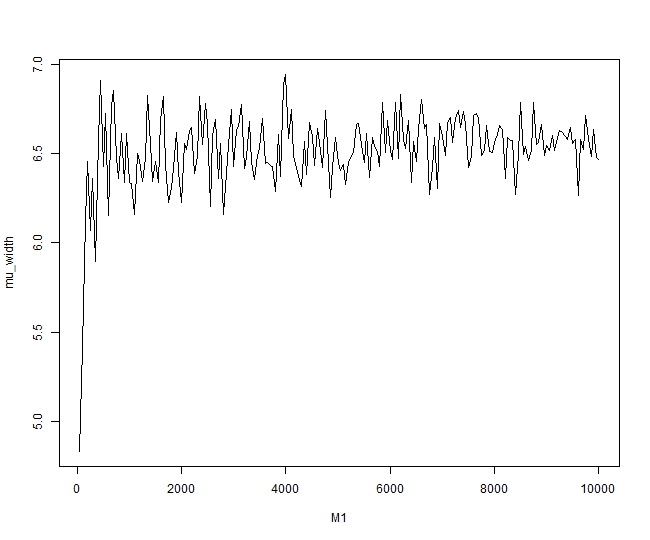
\includegraphics[width = \textwidth]{./Codes/mu_10_2.jpg}
    	\caption{$n = 10, \lambda = 2$}
    	\end{subfigure}%
    	\begin{subfigure}[b]{0.5\textwidth}
    	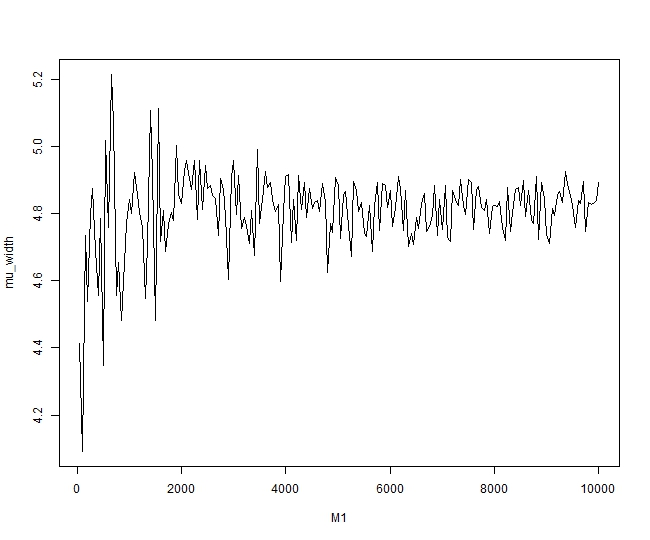
\includegraphics[width = \textwidth]{./Codes/mu_10_12.jpg}
    	\caption{$n = 10, \lambda = 12$}
    	\end{subfigure}%

    	\begin{subfigure}[b]{0.5\textwidth}
    	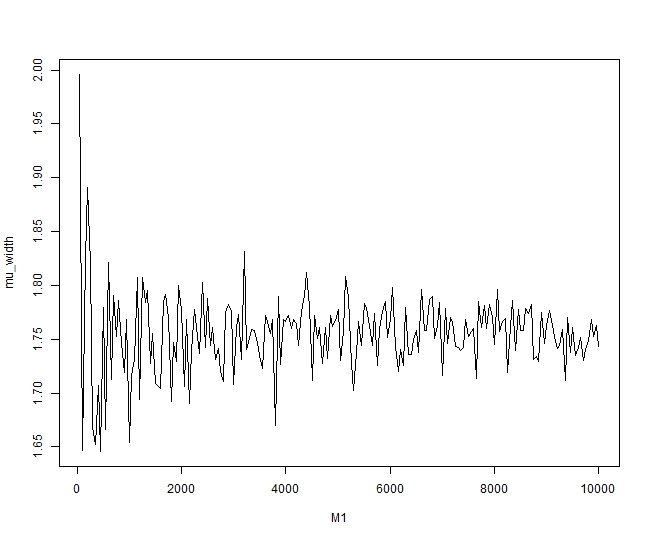
\includegraphics[width = \textwidth]{./Codes/mu_50_8.jpg}
    	\caption{$n = 50, \lambda = 8$}
    	\end{subfigure}%
    	\begin{subfigure}[b]{0.5\textwidth}
    	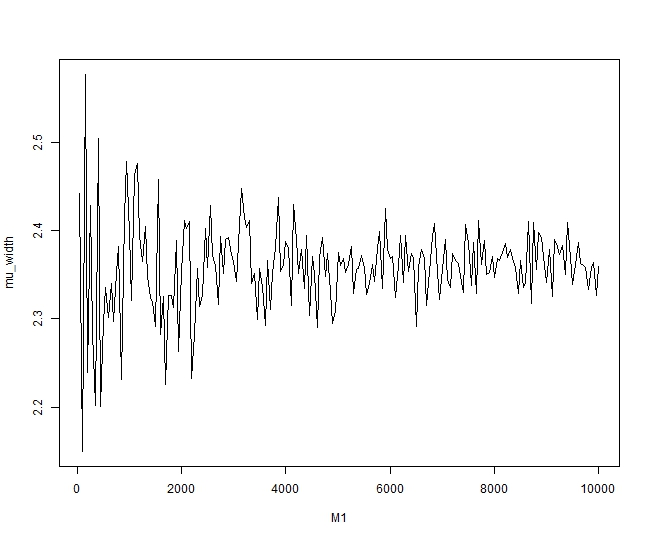
\includegraphics[width = \textwidth]{./Codes/mu_100_4.jpg}
    	\caption{$n = 100, \lambda = 4$}
    	\end{subfigure}%

    	\begin{subfigure}[b]{0.5\textwidth}
    	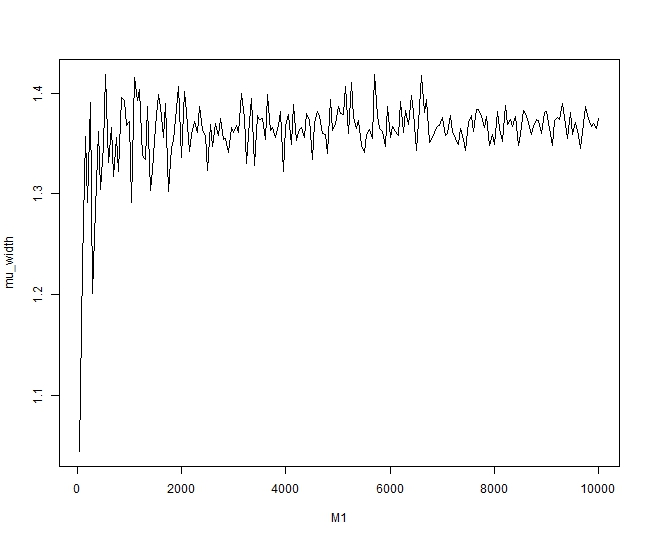
\includegraphics[width = \textwidth]{./Codes/mu_500_2.jpg}
    	\caption{$n = 500, \lambda = 2$}
    	\end{subfigure}%
    	\begin{subfigure}[b]{0.5\textwidth}
    	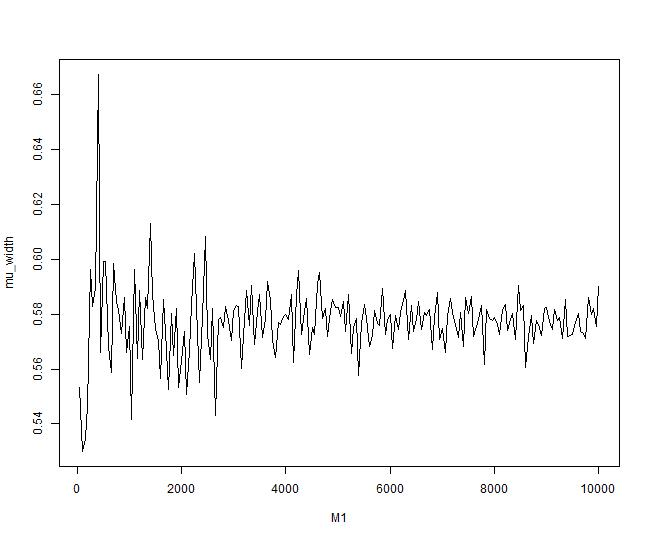
\includegraphics[width = \textwidth]{./Codes/mu_500_12.jpg}
    	\caption{$n = 500, \lambda = 12$}
    	\end{subfigure}
    	\caption{Interval widths for $\mu$ for a series of $M_1$}
    	\label{chooseM1_mu}
    \end{figure}


        \begin{figure}[!htb]
        \centering
    	\begin{subfigure}[b]{0.5\textwidth}
    	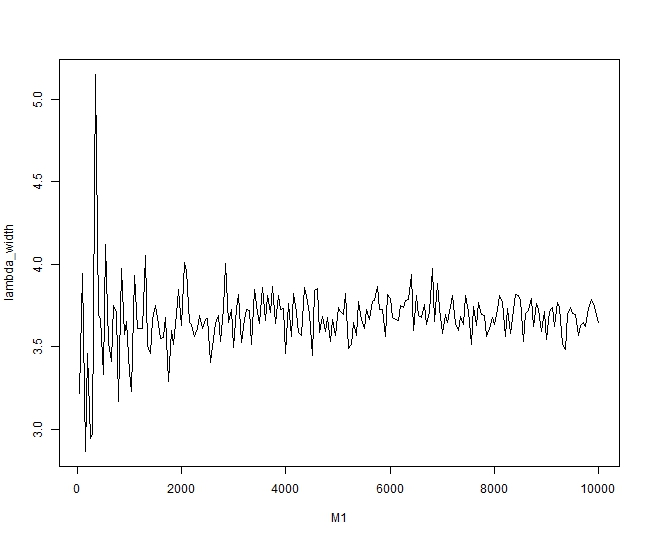
\includegraphics[width = \textwidth]{./Codes/lambda_10_2.jpg}
    	\caption{$n = 10, \lambda = 2$}
    	\end{subfigure}%
    	\begin{subfigure}[b]{0.5\textwidth}
    	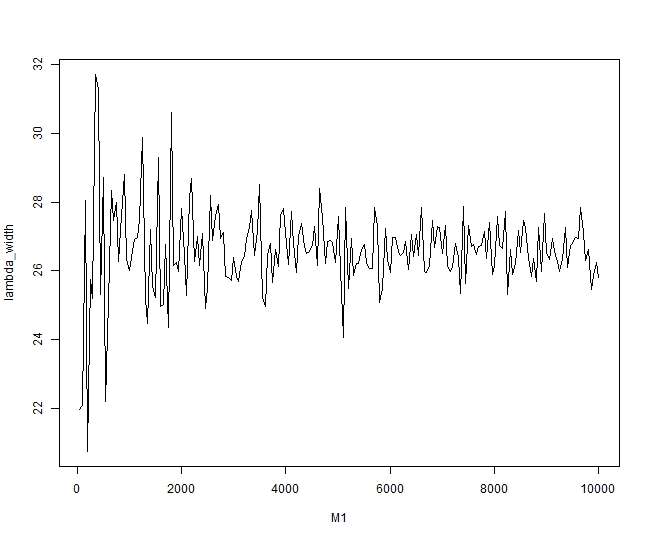
\includegraphics[width = \textwidth]{./Codes/lambda_10_12.jpg}
    	\caption{$n = 10, \lambda = 12$}
    	\end{subfigure}%

    	\begin{subfigure}[b]{0.5\textwidth}
    	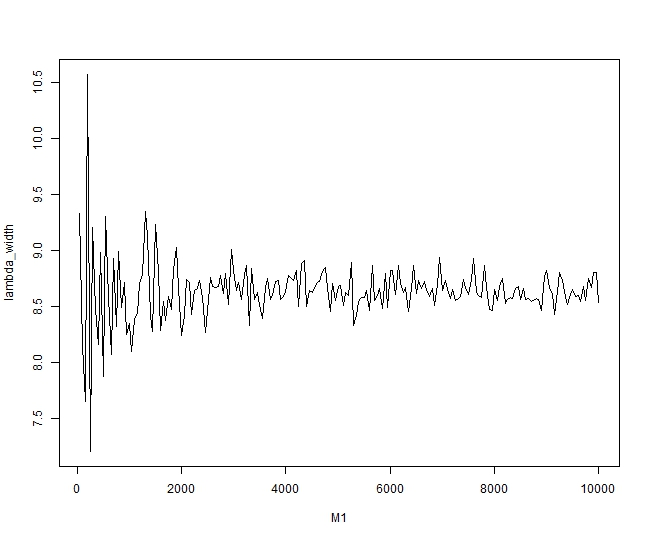
\includegraphics[width = \textwidth]{./Codes/lambda_50_8.jpg}
    	\caption{$n = 50, \lambda = 8$}
    	\end{subfigure}%
    	\begin{subfigure}[b]{0.5\textwidth}
    	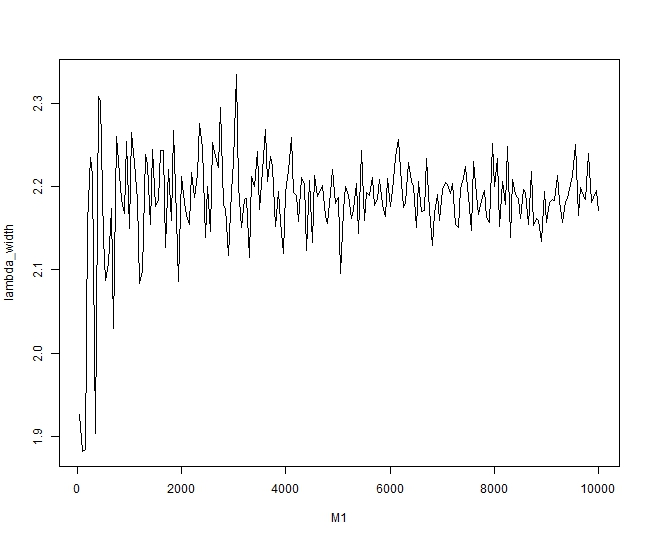
\includegraphics[width = \textwidth]{./Codes/lambda_100_4.jpg}
    	\caption{$n = 100, \lambda = 4$}
    	\end{subfigure}%
    	
    	\begin{subfigure}[b]{0.5\textwidth}
    	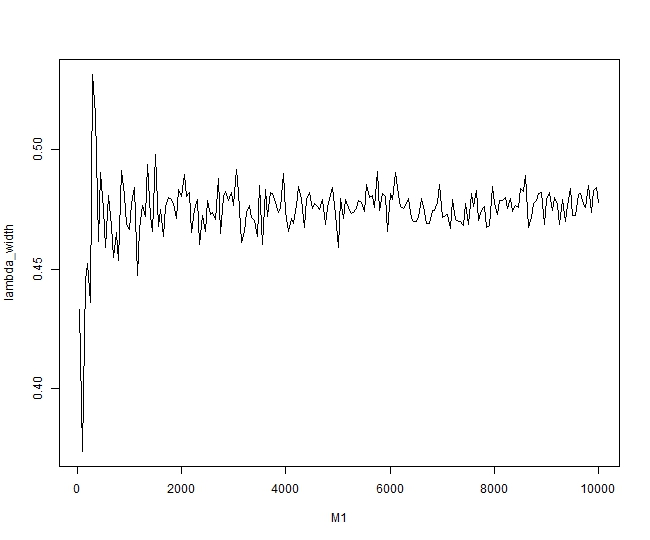
\includegraphics[width = \textwidth]{./Codes/lambda_500_2.jpg}
    	\caption{$n = 500, \lambda = 2$}
    	\end{subfigure}%
    	\begin{subfigure}[b]{0.5\textwidth}
    	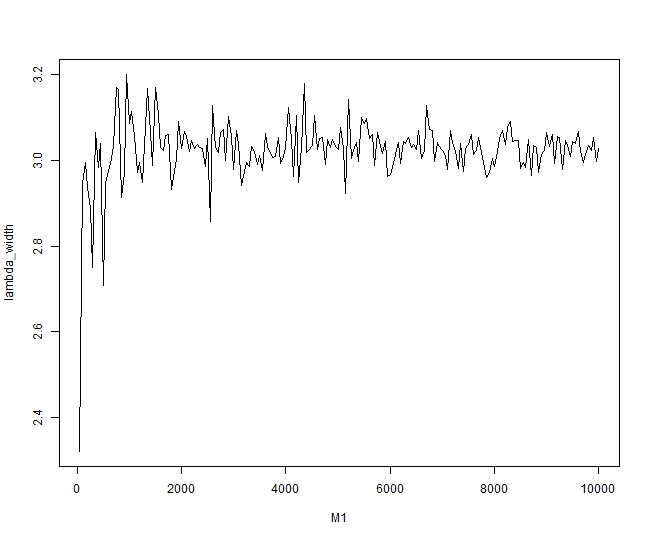
\includegraphics[width = \textwidth]{./Codes/lambda_500_12.jpg}
    	\caption{$n = 500, \lambda = 12$}
    	\end{subfigure}
    	\caption{Interval widths for $\lambda$ for a series of $M_1$}
    	\label{chooseM1_lambda}
    \end{figure}
    \subsection{Comparison of 6 methods in 20 situations}
    The results of comparison of 6 methods in 20 situations are presented in Table \ref{comp}. Each of Table \ref{10_2} to \ref{500_12} is a comparison based on three features of 6 kinds of intervals, where wald represents Wald Theory interval, inv. lrt represents interval from inversion of LRT, boot1 to boot3 represent first 3 bootstrap intervals based on MLE and boot4 represents bootstrap interval based on MME. For the column names, coverage rate, median width and out prob. are MC approximations of actual coverage rate, median of interval width and probability that the interval endpoints fall out of the parameter space.  A discussion about the results is in section \ref{discussion}.

    \begin{table}[!htb]
	\small
		\centering
		\caption{Comparison of different methods}
		\label{comp}
		\begin{subtable}[b]{\textwidth}
		\centering
		\begin{tabular}{l|lll|lll}
		\toprule
        \multirow{2}{*}{Method} & \multicolumn{3}{c|}{$\mu$}      & \multicolumn{3}{c}{$\lambda$}  \\ 
                           & coverage rate & median width & out prob. & coverage rate & median width & out prob. \\
                           \midrule
wald       &0.7908&	7.415596717&	0.3037               &    0.9702&4.53588619634598&0.5324\\
inv. lrt   &0.9267&	61.35652128&	0               &0.9221&4.25027621377186&0\\
boot1      &0.7315&	7.233399848&	0.547               &0.8994&7.51762048562962&1\\
boot2      &0.8566&	8.465186718&	0               &0.9486&3.86520979172964&0\\
boot3      &0.8805&	13.41687309&	0               &0.9486&3.86520953662003&0\\
boot4      &0.6976&	5.699996822&	0.2645               &0.9571&17.6406456091096&1\\
       \bottomrule
       \end{tabular}
       \caption{$n = 10, \lambda = 2$}
       \label{10_2}
       \end{subtable}%

\begin{subtable}[b]{\textwidth}
		\centering
		\begin{tabular}{l|lll|lll}
		\toprule
        \multirow{2}{*}{Method} & \multicolumn{3}{c|}{$\mu$}      & \multicolumn{3}{c}{$\lambda$}  \\ 
                           & coverage rate & median width & out prob. & coverage rate & median width & out prob. \\
                           \midrule
wald       &0.8434	&5.727604814&	0.0358&0.9744	&9.260143039&	0.5444\\    
inv. lrt   &0.9331	&11.70000616&	0     &0.9239	&8.623049065&	0\\
boot1      &0.7979	&5.63221238	&0.1706   &0.9046	&15.2658961	&1\\
boot2      &0.8831	&6.165520751&	0     &0.9492	&7.834264047&	0\\ 
boot3      &0.9198	&8.741260887&	0     &0.9492	&7.834267742&	0\\
boot4      &0.7768	&4.833330351&	0.0749&0.9395	&26.958766	&1\\
       \bottomrule
       \end{tabular}
       \caption{$n = 10, \lambda = 4$}
       \label{10_4}
       \end{subtable}%

       \begin{subtable}[b]{\textwidth}
		\centering
		\begin{tabular}{l|lll|lll}
		\toprule
        \multirow{2}{*}{Method} & \multicolumn{3}{c|}{$\mu$}      & \multicolumn{3}{c}{$\lambda$}  \\ 
                           & coverage rate & median width & out prob. & coverage rate & median width & out prob. \\
                           \midrule
wald      &0.8726&	4.264057063&	1.00E-04	&0.9744	&17.88400597&	0.526\\ 
inv. lrt  &0.9328&	6.276669553&	0	       & 0.929	&16.83232546&	0 \\
boot1     &0.8416&	4.223124743&	0.0063	   & 0.9	&29.77911132&	1 \\
boot2     &0.8943&	4.446041743&	0	       & 0.9531	&15.30432115&	0 \\
boot3     &0.935	&   5.904755356&	0	       & 0.9531	&15.30431668&	0 \\
boot4     &0.8264&	3.823110389&	0.0067	   & 0.9251	&42.96361749&	1 \\
       \bottomrule
       \end{tabular}
       \caption{$n = 10, \lambda = 8$}
       \label{10_8}
       \end{subtable}%

       \begin{subtable}[b]{\textwidth}
		\centering
		\begin{tabular}{l|lll|lll}
		\toprule
        \multirow{2}{*}{Method} & \multicolumn{3}{c|}{$\mu$}      & \multicolumn{3}{c}{$\lambda$}  \\ 
                           & coverage rate & median width & out prob. & coverage rate & median width & out prob. \\
                           \midrule
wald      &0.8805	&3.49373368	    &0         &0.9702	&27.41036385&	0.5378\\
inv. lrt  &0.928	&4.597509056	&0         &0.9242	&25.62849256&	0     \\
boot1     &0.86 	&3.464404455	&2.00E-04  &0.8981	&45.38770272&	1     \\
boot2     &0.8928	&3.5808356	    &0         &0.9455	&23.30346956&	0     \\
boot3     &0.9361	&4.631275417	&0         &0.9455	&23.30346943&	0     \\
boot4     &0.8443	&3.233008213	&0.0011    &0.9198	&59.11760296&	1     \\
       \bottomrule
       \end{tabular}
       \caption{$n = 10, \lambda = 12$}
       \label{10_12}
       \end{subtable}%

        \begin{subtable}[b]{\textwidth}
		\centering
		\begin{tabular}{l|lll|lll}
		\toprule
        \multirow{2}{*}{Method} & \multicolumn{3}{c|}{$\mu$}      & \multicolumn{3}{c}{$\lambda$}  \\ 
                           & coverage rate & median width & out prob. & coverage rate & median width & out prob. \\
                           \midrule
wald      &0.8671	&5.538234106&	0.0035 &0.9706	&2.536000396	&0.054 \\
inv. lrt  &0.9404	&9.168454773&	0      &0.934	&2.404849449	&0     \\
boot1     &0.8277	&5.459853571&	0.0653 &0.9177	&2.959375503	&0.6164\\
boot2     &0.9088	&5.915407717&	0      &0.943	&2.309046025	&0     \\
boot3     &0.9072	&7.370414469&	0      &0.943	&2.309045453	&0     \\
boot4     &0.8071	&4.704869547&	0.0418 &0.9343	&7.124359388	&1     \\
       \bottomrule
       \end{tabular}
       \caption{$n = 25, \lambda = 2$}
       \label{25_2}
       \end{subtable}%
       \end{table}
       \begin{table}
       \ContinuedFloat
        \begin{subtable}[b]{\textwidth}
		\centering
		\begin{tabular}{l|lll|lll}
		\toprule
        \multirow{2}{*}{Method} & \multicolumn{3}{c|}{$\mu$}      & \multicolumn{3}{c}{$\lambda$}  \\ 
                           & coverage rate & median width & out prob. & coverage rate & median width & out prob. \\
                           \midrule
wald      &0.8965	&4.051324848	&0      &0.9726	&5.073104115 &0.0487\\
inv. lrt  &0.9438	&5.184324773	&0      &0.943	&4.810284695 &0     \\
boot1     &0.8694	&4.002785638	&0      &0.92	&5.922671805 &0.6135\\
boot2     &0.9227	&4.186454539	&0      &0.9504	&4.628273344 &0     \\
boot3     &0.9284	&4.874075379	&0      &0.9504	&4.628272115 &0     \\
boot4     &0.8528	&3.654406313	&0.0016 &0.9326	&10.95103051 &1     \\
       \bottomrule
       \end{tabular}
       \caption{$n = 25, \lambda = 4$}
       \label{25_4}
       \end{subtable}%

        \begin{subtable}[b]{\textwidth}
		\centering
		\begin{tabular}{l|lll|lll}
		\toprule
        \multirow{2}{*}{Method} & \multicolumn{3}{c|}{$\mu$}      & \multicolumn{3}{c}{$\lambda$}  \\ 
                           & coverage rate & median width & out prob. & coverage rate & median width & out prob. \\
                           \midrule
wald      &0.9149	&2.914383562	&0  &0.9709	&10.06976682	&0.0476\\
inv. lrt  &0.9408	&3.351924594	&0  &0.9441	&9.580044484	&0     \\
boot1     &0.8979	&2.895781339	&0  &0.9131	&11.83754515	&0.6219\\
boot2     &0.9269	&2.962903395	&0  &0.9496	&9.210312148	&0     \\
boot3     &0.9378	&3.320163792	&0  &0.9496	&9.210314701	&0     \\
boot4     &0.8818	&2.742464318	&0  &0.9225	&17.67656694	&1     \\
       \bottomrule
       \end{tabular}
       \caption{$n = 25, \lambda = 8$}
       \label{25_8}
       \end{subtable}%

        \begin{subtable}[b]{\textwidth}
		\centering
		\begin{tabular}{l|lll|lll}
		\toprule
        \multirow{2}{*}{Method} & \multicolumn{3}{c|}{$\mu$}      & \multicolumn{3}{c}{$\lambda$}  \\ 
                           & coverage rate & median width & out prob. & coverage rate & median width & out prob. \\
                           \midrule
wald      &0.9216	&2.406498653	&0 &0.9721	&14.99667068	&0.0493\\
inv. lrt  &0.9451	&2.67450462	    &0 &0.9438	&14.31288196	&0     \\
boot1     &0.9099	&2.399513123	&0 &0.9173	&17.61077342	&0.6023\\
boot2     &0.9304	&2.433127394	&0 &0.9491	&13.78011734	&0     \\
boot3     &0.9439	&2.688899586	&0 &0.9491	&13.78011745	&0     \\
boot4     &0.9006	&2.296748259	&0 &0.9272	&24.12421905	&1     \\
       \bottomrule
       \end{tabular}
       \caption{$n = 25, \lambda = 12$}
       \label{25_12}
       \end{subtable}%

        \begin{subtable}[b]{\textwidth}
		\centering
		\begin{tabular}{l|lll|lll}
		\toprule
        \multirow{2}{*}{Method} & \multicolumn{3}{c|}{$\mu$}      & \multicolumn{3}{c}{$\lambda$}  \\ 
                           & coverage rate & median width & out prob. & coverage rate & median width & out prob. \\
                           \midrule
wald      & 0.8994	&4.116607908	&0      & 0.971	  &1.691113612	&0     \\ 
inv. lrt  & 0.9473	&5.178413337	&0      & 0.9451  &1.628672324	&0     \\ 
boot1     & 0.8695	&4.084247902	&0      & 0.93	  &1.801906403	&0     \\ 
boot2     & 0.9279	&4.272589653	&0      & 0.946	  &1.595437725	&0     \\ 
boot3     & 0.9275	&4.810280159	&0      & 0.946	  &1.595437663	&0     \\ 
boot4     & 0.8538	&3.712295527	&0.0025 & 0.9296  &4.403723433	&0.9547\\ 
       \bottomrule
       \end{tabular}
       \caption{$n = 50, \lambda = 2$}
       \label{50_2}
       \end{subtable}%

        \begin{subtable}[b]{\textwidth}
		\centering
		\begin{tabular}{l|lll|lll}
		\toprule
        \multirow{2}{*}{Method} & \multicolumn{3}{c|}{$\mu$}      & \multicolumn{3}{c}{$\lambda$}  \\ 
                           & coverage rate & median width & out prob. & coverage rate & median width & out prob. \\
                           \midrule
wald      & 0.9218	&2.987688288	&0 & 0.9721	&3.361219247	&0     \\
inv. lrt  & 0.9482	&3.368235802	&0 & 0.95	&3.248136046	&0     \\
boot1     & 0.9056	&2.969777113	&0 & 0.9299	&3.592543563	&0     \\
boot2     & 0.9348	&3.039788797	&0 & 0.9518	&3.181596087	&0     \\
boot3     & 0.9406	&3.294773231	&0 & 0.9518	&3.181595303	&0     \\
boot4     & 0.8942	&2.788904487	&0 & 0.9324	&6.828555914	&0.5793\\
       \bottomrule
       \end{tabular}
       \caption{$n = 50, \lambda = 4$}
       \label{50_4}
       \end{subtable}%  
       \end{table}
       \begin{table}
       \ContinuedFloat
        \begin{subtable}[b]{\textwidth}
		\centering
		\begin{tabular}{l|lll|lll}
		\toprule
        \multirow{2}{*}{Method} & \multicolumn{3}{c|}{$\mu$}      & \multicolumn{3}{c}{$\lambda$}  \\ 
                           & coverage rate & median width & out prob. & coverage rate & median width & out prob. \\
                           \midrule
wald      & 0.9303	&2.131000046	&0 &0.9722	&6.764364997&	0     \\
inv. lrt  & 0.9449	&2.281818834	&0 &0.9456	&6.514737471&	0     \\
boot1     & 0.9196	&2.124543679	&0 &0.9297	&7.205545945&	0     \\
boot2     & 0.9357	&2.150266853	&0 &0.9489	&6.385045737&	0     \\
boot3     & 0.9427	&2.276742616	&0 &0.9489	&6.38504706	&   0     \\
boot4     & 0.9138	&2.045281224	&0 &0.9354	&11.10872079&	0.0495\\
       \bottomrule
       \end{tabular}
       \caption{$n = 50, \lambda = 8$}
       \label{50_8}
       \end{subtable}%  

        \begin{subtable}[b]{\textwidth}
		\centering
		\begin{tabular}{l|lll|lll}
		\toprule
        \multirow{2}{*}{Method} & \multicolumn{3}{c|}{$\mu$}      & \multicolumn{3}{c}{$\lambda$}  \\ 
                           & coverage rate & median width & out prob. & coverage rate & median width & out prob. \\
                           \midrule
wald      & 0.9325	&1.748060489	&0 & 0.9725	&10.10319374    &	2.00E-04\\
inv. lrt  & 0.9431	&1.841761131	&0 & 0.9459	&9.752976421    &	0       \\
boot1     & 0.9258	&1.7414177	    &0 & 0.9305	&10.78126849    &	0       \\  
boot2     & 0.9344	&1.75516099	    &0 & 0.9488	&9.549431077    &	0       \\  
boot3     & 0.9421	&1.845891662	&0 & 0.9488	&9.54943602	    &   0       \\  
boot4     & 0.92	&1.696687033	&0 & 0.9349	&15.12174617    &	0.0023  \\
       \bottomrule
       \end{tabular}
       \caption{$n = 50, \lambda = 12$}
       \label{50_12}
       \end{subtable}%  

        \begin{subtable}[b]{\textwidth}
		\centering
		\begin{tabular}{l|lll|lll}
		\toprule
        \multirow{2}{*}{Method} & \multicolumn{3}{c|}{$\mu$}      & \multicolumn{3}{c}{$\lambda$}  \\ 
                           & coverage rate & median width & out prob. & coverage rate & median width & out prob. \\
                           \midrule
wald      & 0.9236	&3.011063163  &	0        & 0.9706	&1.161093068	&0     \\
inv. lrt  & 0.9464	&3.360407941  &	0        & 0.9444	&1.129581016	&0     \\
boot1     & 0.9039	&2.996376339  &	0        & 0.9373	&1.184256781	&0     \\
boot2     & 0.9374	&3.068666046  &	0        & 0.9489	&1.115444506	&0     \\
boot3     & 0.9353	&3.263857369  &	0        & 0.9489	&1.115444507	&0     \\
boot4     & 0.8909	&2.81374028	  & 1.00E-04 & 0.9347	&2.978213938	&0.1702\\
       \bottomrule
       \end{tabular}
       \caption{$n = 100, \lambda = 2$}
       \label{100_2}
       \end{subtable}%

        \begin{subtable}[b]{\textwidth}
		\centering
		\begin{tabular}{l|lll|lll}
		\toprule
        \multirow{2}{*}{Method} & \multicolumn{3}{c|}{$\mu$}      & \multicolumn{3}{c}{$\lambda$}  \\ 
                           & coverage rate & median width & out prob. & coverage rate & median width & out prob. \\
                           \midrule
wald      & 0.9393	&2.148338512   	&0 & 0.9715	&2.337690861	&0     \\
inv. lrt  & 0.9506	&2.27745012	    &0 & 0.9456	&2.264702465	&0     \\
boot1     & 0.9257	&2.136277973   	&0 & 0.9369	&2.377011311	&0     \\
boot2     & 0.9449	&2.162477535   	&0 & 0.9484	&2.240657081	&0     \\
boot3     & 0.9449	&2.252973071   	&0 & 0.9484	&2.240657293	&0     \\
boot4     & 0.9182	&2.062179009   	&0 & 0.9407	&4.637655957	&0.0023\\
       \bottomrule
       \end{tabular}
       \caption{$n = 100, \lambda = 4$}
       \label{100_4}
       \end{subtable}%

        \begin{subtable}[b]{\textwidth}
		\centering
		\begin{tabular}{l|lll|lll}
		\toprule
        \multirow{2}{*}{Method} & \multicolumn{3}{c|}{$\mu$}      & \multicolumn{3}{c}{$\lambda$}  \\ 
                           & coverage rate & median width & out prob. & coverage rate & median width & out prob. \\
                           \midrule
wald      & 0.9399	&1.530069999	&0 & 0.9715	&4.665225374   	&0 \\
inv. lrt  & 0.9507	&1.581786207	&0 & 0.9476	&4.525775706   	&0 \\
boot1     & 0.934	&1.524664931	&0 & 0.94	&4.739872744   	&0 \\
boot2     & 0.9447	&1.533174131	&0 & 0.9481	&4.46553391	    &0 \\
boot3     & 0.9493	&1.577987392	&0 & 0.9481	&4.465533898   	&0 \\
boot4     & 0.9281	&1.489659246	&0 & 0.9403	&7.522671314   	&0 \\
       \bottomrule
       \end{tabular}
       \caption{$n = 100, \lambda = 8$}
       \label{100_8}
       \end{subtable}% 
       \end{table}

       \begin{table}
       \ContinuedFloat
        \begin{subtable}[b]{\textwidth}
		\centering
		\begin{tabular}{l|lll|lll}
		\toprule
        \multirow{2}{*}{Method} & \multicolumn{3}{c|}{$\mu$}      & \multicolumn{3}{c}{$\lambda$}  \\ 
                           & coverage rate & median width & out prob. & coverage rate & median width & out prob. \\
                           \midrule
wald      & 0.9417	&1.250315505	&0 & 0.9714	&6.914885138	&0\\
inv. lrt  & 0.949	&1.282844649	&0 & 0.9495	&6.759021307	&0\\
boot1     & 0.9379	&1.246129311	&0 & 0.9395	&7.090872634	&0\\
boot2     & 0.9438	&1.251665971	&0 & 0.9504	&6.680855241	&0\\
boot3     & 0.9485	&1.283024333	&0 & 0.9504	&6.680848082	&0\\
boot4     & 0.9317	&1.223816082	&0 & 0.9399	&10.17049293	&0\\
       \bottomrule
       \end{tabular}
       \caption{$n = 100, \lambda = 12$}
       \label{100_12}
       \end{subtable}%

        \begin{subtable}[b]{\textwidth}
		\centering
		\begin{tabular}{l|lll|lll}
		\toprule
        \multirow{2}{*}{Method} & \multicolumn{3}{c|}{$\mu$}      & \multicolumn{3}{c}{$\lambda$}  \\ 
                           & coverage rate & median width & out prob. & coverage rate & median width & out prob. \\
                           \midrule
wald      & 0.9451	&1.379903433	 &0 & 0.9723	&0.503826117	&0 \\
inv. lrt  & 0.9509	&1.40921584	     &0 & 0.9464	&0.497522219	&0 \\
boot1     & 0.9384	&1.375420546	 &0 & 0.9441	&0.501491495	&0 \\
boot2     & 0.9478	&1.382673706	 &0 & 0.9458	&0.495552047	&0 \\
boot3     & 0.9473	&1.399477573	 &0 & 0.9458	&0.495552084	&0 \\
boot4     & 0.9337	&1.352265457	 &0 & 0.9428	&1.359178854	&0 \\
       \bottomrule
       \end{tabular}
       \caption{$n = 500, \lambda = 2$}
       \label{500_2}
       \end{subtable}%   


        \begin{subtable}[b]{\textwidth}
		\centering
		\begin{tabular}{l|lll|lll}
		\toprule
        \multirow{2}{*}{Method} & \multicolumn{3}{c|}{$\mu$}      & \multicolumn{3}{c}{$\lambda$}  \\ 
                           & coverage rate & median width & out prob. & coverage rate & median width & out prob. \\
                           \midrule
wald      & 0.9451	&0.976933623	&0  & 0.9746	&1.007529936 &	0\\
inv. lrt  & 0.95	&0.987981173	&0  & 0.9488	&0.995081084 &	0\\
boot1     & 0.9431	&0.973634767	&0  & 0.9477	&1.002816785 &	0\\
boot2     & 0.9468	&0.976019364	&0  & 0.949	    &0.991152256 &	0\\
boot3     & 0.9489	&0.983498117	&0  & 0.949	    &0.991152432 &	0\\
boot4     & 0.9407	&0.966411182	&0  & 0.9474	&2.095926752 &	0\\
       \bottomrule
       \end{tabular}
       \caption{$n = 500, \lambda = 4$}
       \label{500_4}
       \end{subtable}% 

        \begin{subtable}[b]{\textwidth}
		\centering
		\begin{tabular}{l|lll|lll}
		\toprule
        \multirow{2}{*}{Method} & \multicolumn{3}{c|}{$\mu$}      & \multicolumn{3}{c}{$\lambda$}  \\ 
                           & coverage rate & median width & out prob. & coverage rate & median width & out prob. \\
                           \midrule
wald      & 0.9484	&0.692079344	&0 & 0.9701	&2.008704726	&0\\
inv. lrt  & 0.9474	&0.696625278	&0 & 0.9472	&1.988841356	&0\\
boot1     & 0.9444	&0.690128888	&0 & 0.9447	&2.002078022	&0\\
boot2     & 0.9475	&0.690995417	&0 & 0.9463	&1.97850184	&0\\
boot3     & 0.9464	&0.695246151	&0 & 0.9463	&1.978501088	&0\\
boot4     & 0.9453	&0.686891841	&0 & 0.9455	&3.326968948	&0\\
       \bottomrule
       \end{tabular}
       \caption{$n = 500, \lambda = 8$}
       \label{500_8}
       \end{subtable}% 

        \begin{subtable}[b]{\textwidth}
		\centering
		\begin{tabular}{l|lll|lll}
		\toprule
        \multirow{2}{*}{Method} & \multicolumn{3}{c|}{$\mu$}      & \multicolumn{3}{c}{$\lambda$}  \\ 
                           & coverage rate & median width & out prob. & coverage rate & median width & out prob. \\
                           \midrule
wald      & 0.9439	&0.564066402	&0 & 0.9731	&3.034407101	&0\\
inv. lrt  & 0.9463	&0.566843921	&0 & 0.9455	&2.98750447	&0\\
boot1     & 0.9422	&0.562103595	&0 & 0.9467	&3.012273927	&0\\
boot2     & 0.9441	&0.562551002	&0 & 0.9452	&2.976193417	&0\\
boot3     & 0.9456	&0.565621322	&0 & 0.9452	&2.976193516	&0\\
boot4     & 0.9412	&0.561039752	&0 & 0.9476	&4.456659554	&0\\
       \bottomrule
       \end{tabular}
       \caption{$n = 500, \lambda = 12$}
       \label{500_12}
       \end{subtable}% 


       \end{table}

       \clearpage
	\section{Discussion and Conclusions}\label{discussion}

	When $n = 10$, we look at Table \ref{10_2} - \ref{10_12}. We find that for all $\lambda = 2, 4, 8, 12$, wald, boot1 and boot4 have a pretty large out prob., and out prob. wrt $\lambda$ does not change a lot as $\lambda$ increases. What's more, boot1 and boot4 has larger median width wrt $\lambda$ then other methods for all $\lambda = 2, 4, 8, 12$. The method inv. lrt has a significant larger median width wrt $\mu$ when $\lambda$ is small. But it drops a lot as $\lambda$ increases. Methods boot2 and boot3 has better performance than others when $\lambda = 2, 4$. Both of them has 0 out. prob, while boot3 has a little larger coverage rate and median width than boot2. So in this case boot2 and boot3 are probably two good choices. When $\lambda = 8, 12$, inv. lrt and boot3 have similar coverage rate and median width, while boot2's coverage rate is still below 90\%, hence I think inv. lrt and boot3 are two good choices now. And a common pattern for all methods is coverage rate, median width and out prob. wrt $\mu$ are decreasing as $\lambda$ increases, when median with wrt $\lambda$ is increasing.

	When $n = 25$, for Table \ref{25_2} - \ref{25_12}, similar patterns can be found as $\lambda$ increases. Method boot1 still has larger median width wrt $\lambda$, but the difference is not much. Method boot4 still has a significant larger median width wrt $\lambda$. And boot1, boot4 still has large out. prob wrt $\lambda$, while that of wald is now that big now. However, coverage rate wrt $\mu$ of wald is smaller than inv. lrt, boot2 and boo3. Method inv. lrt, boot2 and boot3 have coverage rate close to 95\%, and there is not big difference in them wrt $\lambda$. When $\lambda$ is small, inv. lrt has a larger coverage rate as well as a bigger median width, boot2 and boot3 has similar coverage rate. while boot2 has smaller median with wrt $\mu$. When $\lambda$ is large, inv. lrt and boot3 have similar coverage rate and median width, while the coverage rate and median width are both smaller. So when $\lambda$ is large ($\lambda = 8, 12$), inv. lrt, boot2, boot3 are all possible choices. And for $\lambda$ small ($\lambda = 2, 4$), I would prefer inv. lrt, boot2.

	When $n = 50$, in Table \ref{50_2} - \ref{50_12}, we can see only boot4 has non-zero out. prob wrt $\lambda$. It is still big when $\lambda = 2, 4$, but is pretty small when $\lambda = 8, 12$. However, the median width wrt $\lambda$ by boot4 is still big. When $\lambda = 2$, inv. irt has larger coverage rate that is close to 95\% and bigger median width wrt $\mu$. boot2 and boot3 has similar coverage rate while boot2 has smaller median width. When $\lambda = 4, 8, 12$, inv. lrt and boot3 have similar coverage rate and median width, while boot2 has smaller coverage rate and smaller median width, but is still close to 95\%. Method wald also has coverage rate wrt $\mu$ close to 95\% and good median width when $\lambda = 4, 8, 12$, but the coverage rate is over 95\% with large median width wrt $\lambda$, which is not good compared with other methods providing almost exact 95\% wrt $\lambda$. Hence I would prefer boot2, inv. lrt for $\lambda =2$ and inv.lrt, boot2, boot3 for $\lambda = 4, 8, 12$. 

	When $n = 100$, in Table \ref{100_2} - \ref{100_12}, boot4 still has a larger median width wrt $\lambda$ than other methods, so it is not a good choice for any $\lambda = 2, 4, 8, 12.$ For $\lambda = 2, 4$, inv. lrt has a coverage rate closer to 95\% but a bigger median width. Method boot2 and boot3 also provide good coverage rate and smaller median width.  And for $\lambda = 8 ,12$, inv. lrt and boot3 have similar coverage rate and median width, and boot2 has slightly smaller coverage rate and median width. Method boot1's coverage rate wrt $\mu$ in this case is not big enough for all $\lambda = 2, 4, 8, 12$ compared to other methods, and coverage rate wrt $\mu$ by wald is bigger but not as good as those of inv. lrt, boot2 and boot3. Also, the coverage rate wrt $\lambda$ by wald is over 97\% with a bigger median width, which is better compared to more exact interval with proper median width. So I would prefer inv. lrt, boot2, boot3 here for all $\lambda = 2, 4, 8, 12$. 

	When $n = 500$, in Table \ref{500_2} to \ref{500_12}, we can see the median width wrt $\lambda$ by boot4 is still too big compared to other methods. Also, in this case, although wald still gives coverage rate around 97\% wrt $\lambda$, the median width is close to other methods. And it also gives pretty good coverage rate and median width wrt $\mu$. Hence for here wald is also a good choice now. For $\lambda = 2$, boot1's coverage rate wrt $\mu$ is bit small compared to other methods with almost the same median width. And for $\lambda = 4, 8, 12$, inv. lrt, boot1, boot2 and boot3 have similar coverage rate and median width wrt $\mu$ and $\lambda$, and wald also has similar values wrt $\mu$ with these methods. Hence for $\lambda = 2$, wald, inv. lrt, boot2, boot3 are good choices. For $\lambda = 4, 8, 12$, all but boot4 are good choices.

	A summary of preferred methods are shown in Table \ref{preffered}. In Table \ref{preffered} we can see boot2 is always a preferred one. It might not be the best in all cases but it is at least appropriate in all situations. Method boot3 is also always preferred in situations when $\lambda \geq 8$ and $n \geq 100$. It is not a choice when $(n, \lambda) \in \{(25, 2), (25, 4), (50, 2), (50, 4)\}$ because we find boot2 is better in these cases. Although it is not a preferred one, boot3 might still be good to use in these cases. When $n = 10$, boot3 is also preferred. We also find inv. lrt in all situation other than $n=10, \lambda = 2$ and $n = 10, \lambda = 4$. So inv. lrt is a good choice when $n$ and $\lambda$ are not small at the same time. When $n$ is large, we find all methods but boot4 are all good choices. In conclusion, boot2 and boot3 can handle almost all situations; inv. lrt is good when $n$ and $\lambda$ are not simultaneously small; and for $n$ large, all methods but boot4 are good.

	\begin{table}[!htb]
	\caption{Preferred Methods in different situations}
	\label{preffered}
	\begin{tabularx}{\textwidth}{|c|X|X|X|X|}
	\hline
	 \diagbox{$\lambda$}{$n$}& 2 & 4 & 8 & 12\\ \hline
	 10 & boot2, boot3 & boot2, boot3 & inv. lrt, boot3 & inv. lrt, boot3\\ \hline
	 25 &  inv. lrt, boot2 & inv. lrt, boot2 & inv. lrt, boot2, boot3 & inv. lrt, boot2, boot3\\\hline
	 50 &  inv. lrt, boot2 & inv. lrt, boot2 & inv. lrt, boot2, boot3 & inv. lrt, boot2, boot3\\\hline
	 100 & inv. lrt, boot2, boot3 & inv. lrt, boot2, boot3 & inv. lrt, boot2, boot3 & inv. lrt, boot2, boot3 \\ \hline
	 500 & wald, inv. lrt, boot2, boot3 & wald, inv. lrt, boot1, boot2, boot3 & wald, inv. lrt, boot1, boot2, boot3 & wald, inv. lrt, boot1, boot2, boot3\\ \hline
	\end{tabularx}
	\end{table}	

	\newpage



\begin{appendix}
\section*{Appendix: selection of R Codes}
\textbf{All functions:}
\lstinputlisting[language = R]{./Codes/Functions.R}

\textbf{Choosing $M$ when $n = 100, \lambda = 4$:}
\lstinputlisting[language = R]{./Codes/chooseM.R}

\textbf{Choosing $M_1$ when $n=500, \lambda = 2$:}
\lstinputlisting[language = R]{./Codes/chooseM1.R}

\textbf{Comparison when $n = 25, \lambda = 2$:}
\lstinputlisting[language = R]{./Codes/run.R}
\end{appendix}

 	


	
	
	
	\end{document}